\section{How it works}
\subsection{Notation}
The syntax is as follows
\begin{verbatim}
	[assume symbol <expr>]
	[observe (<random proc> <arg> ... <arg>) <const>]
	[predict <expr>]
\end{verbatim}
where \verb!assume!'s are either deterministic or random variables declarations, \verb!observe!'s condition the distribution of the \verb!assume!'d variables and \verb!predict!'s give samples from the posteriors of the corresponding \verb!<expr>!'s.

Probability of an execution trace is
\begin{align}
	\tilde p(\vec y, \vec x) 				&= \prod_{n = 1}^N p(y_n \mid \vec \theta_{t_n}, \vec x_n) \tilde p(\vec x_n \mid \vec x_{n - 1}) \\
	\tilde p(\vec x_n \mid \vec x_{n - 1}) 	&= \prod_{k = 1}^{\vec x_n \setminus \vec x_{n - 1}} p(x_{n, k} \mid \vec \theta_{t_{n, k}}, x_{n, 1:(k - 1)}, \vec x_{n - 1}) \\
	p(y_n \mid \vec \theta_{t_n}, \vec x_n)	&= \text{likelihood of observed output } y_n \\
	\text{tilde}							&= \text{distributions we can only sample from} \\
	y_n										&= n^{\text{th}} \text{ }\mathtt{observe}\text{'d output} \\
	t_n										&= \text{type of } n^{\text{th}} \text{ }\mathtt{observe}\text{'d main }\mathtt{random\ proc} \\
	\vec \theta_{t_n}						&= \text{arguments of } t_n \\
	\vec x_n								&= \text{set of all random procedure application results computed } \nonumber\\
											&\text{before }p(y_n \mid \vec \theta_{t_n}, \vec x_n) \text{ is evaluated. I.e. before the } n^{\text{th}} \text{ observe.}
\end{align}

Whevever a \verb!predict! is called, we want to sample from $\tilde p(\vec x \mid \vec y) \propto \tilde p(\vec y, \vec x)$. A general overview of this can be seen in Figure~\ref{fig:pprog/how/general}.
\begin{figure}[!htb]
\centering
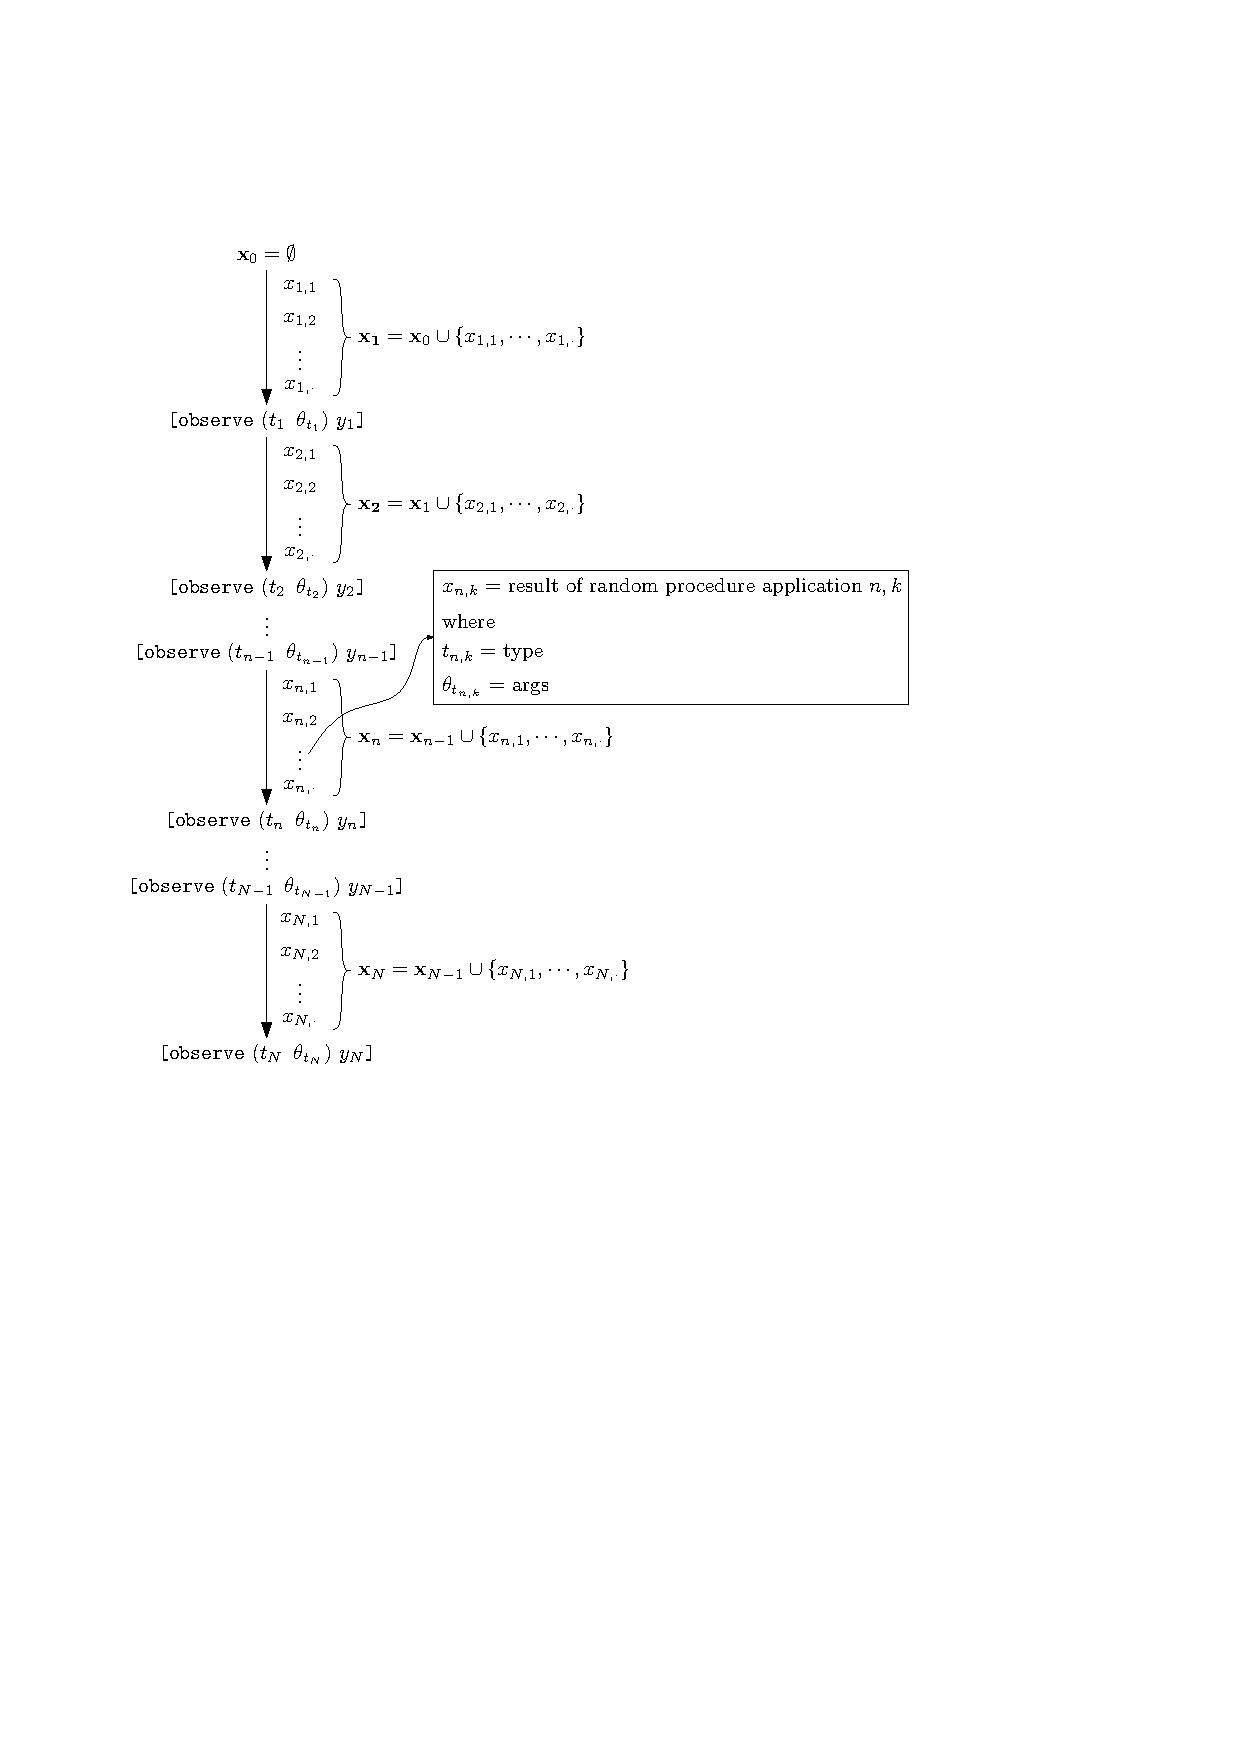
\includegraphics[scale=1]{pprog/how/figures/general/general}
\caption{A general overview of Anglican interpretation.}
\label{fig:pprog/how/general}
\end{figure}

\subsection{Random databse}
This is an Metropolis-Hastings (see Subsection~\ref{subsec:sampling/mcmc-mh/mh}) approach to inference.
\begin{figure}[!htb]
\centering
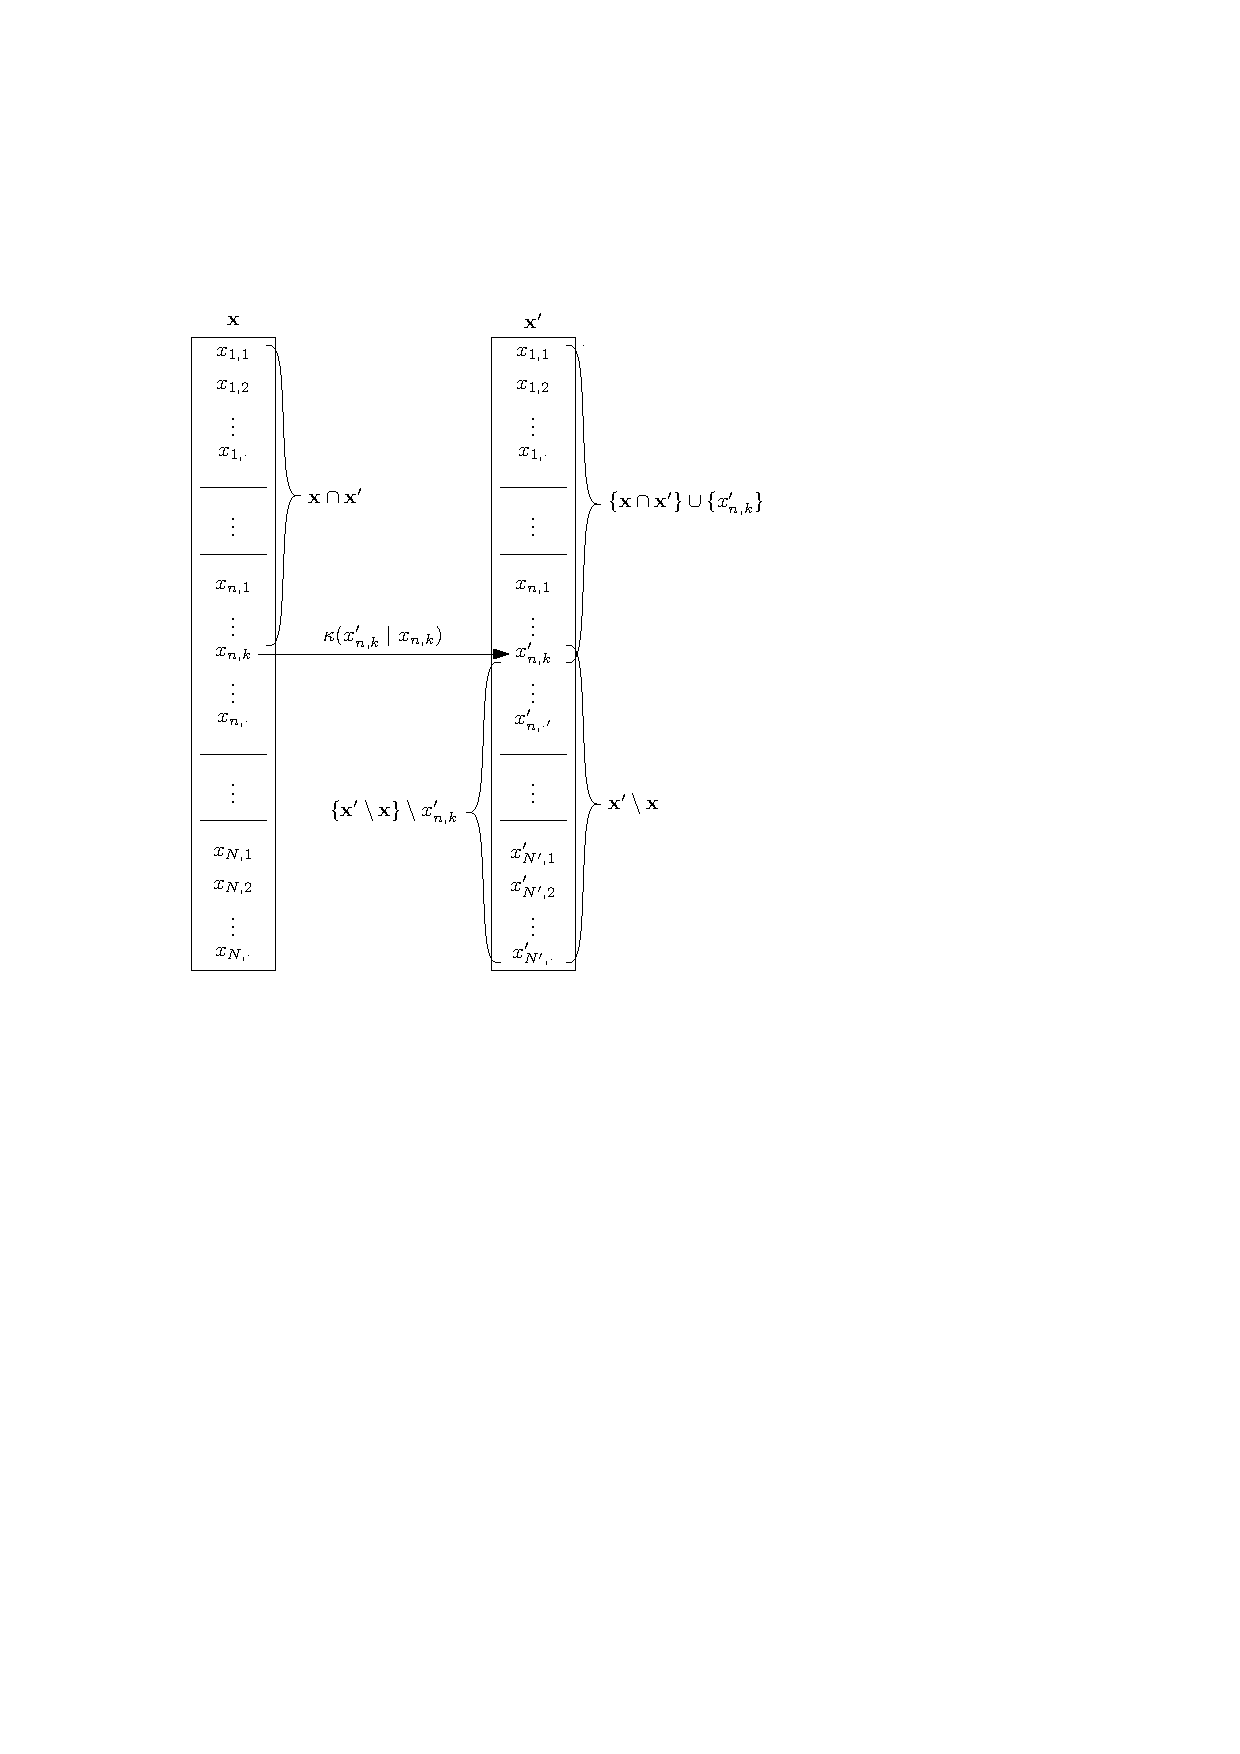
\includegraphics[scale=1]{pprog/how/figures/rdb/rdb}
\caption{Illustration of the RDB algorithm.}
\label{fig:pprog/how/figures/rdb}
\end{figure}

\subsection{Sequential Monte Carlo}
\subsection{Particle Gibbs}
Here, we follow the Particle Gibbs algorithm described in Algorithm~\ref{alg:sampling/pmcmc-pg-pg/pg}. The illustrations are below in Figure~\ref{fig:pprog/how/figures/pgibbs1}, and Figure~\ref{fig:pprog/how/figures/pgibbs2}. Whenever a \verb!predict! is needed, a sample of the posterior of the execution trace can be obtained by sampling from
\begin{equation*}
	\hat p(\mathrm d \vec x_n \mid y_{1:n}, \vec \theta) = \sum_\ell \hat w_n^{(\ell)} \delta_{\vec x_n^{(\ell)}}(\mathrm d \vec x_{n})
\end{equation*}
(This is \emph{with} the retained particle).

\begin{figure}[!htb]
\centering
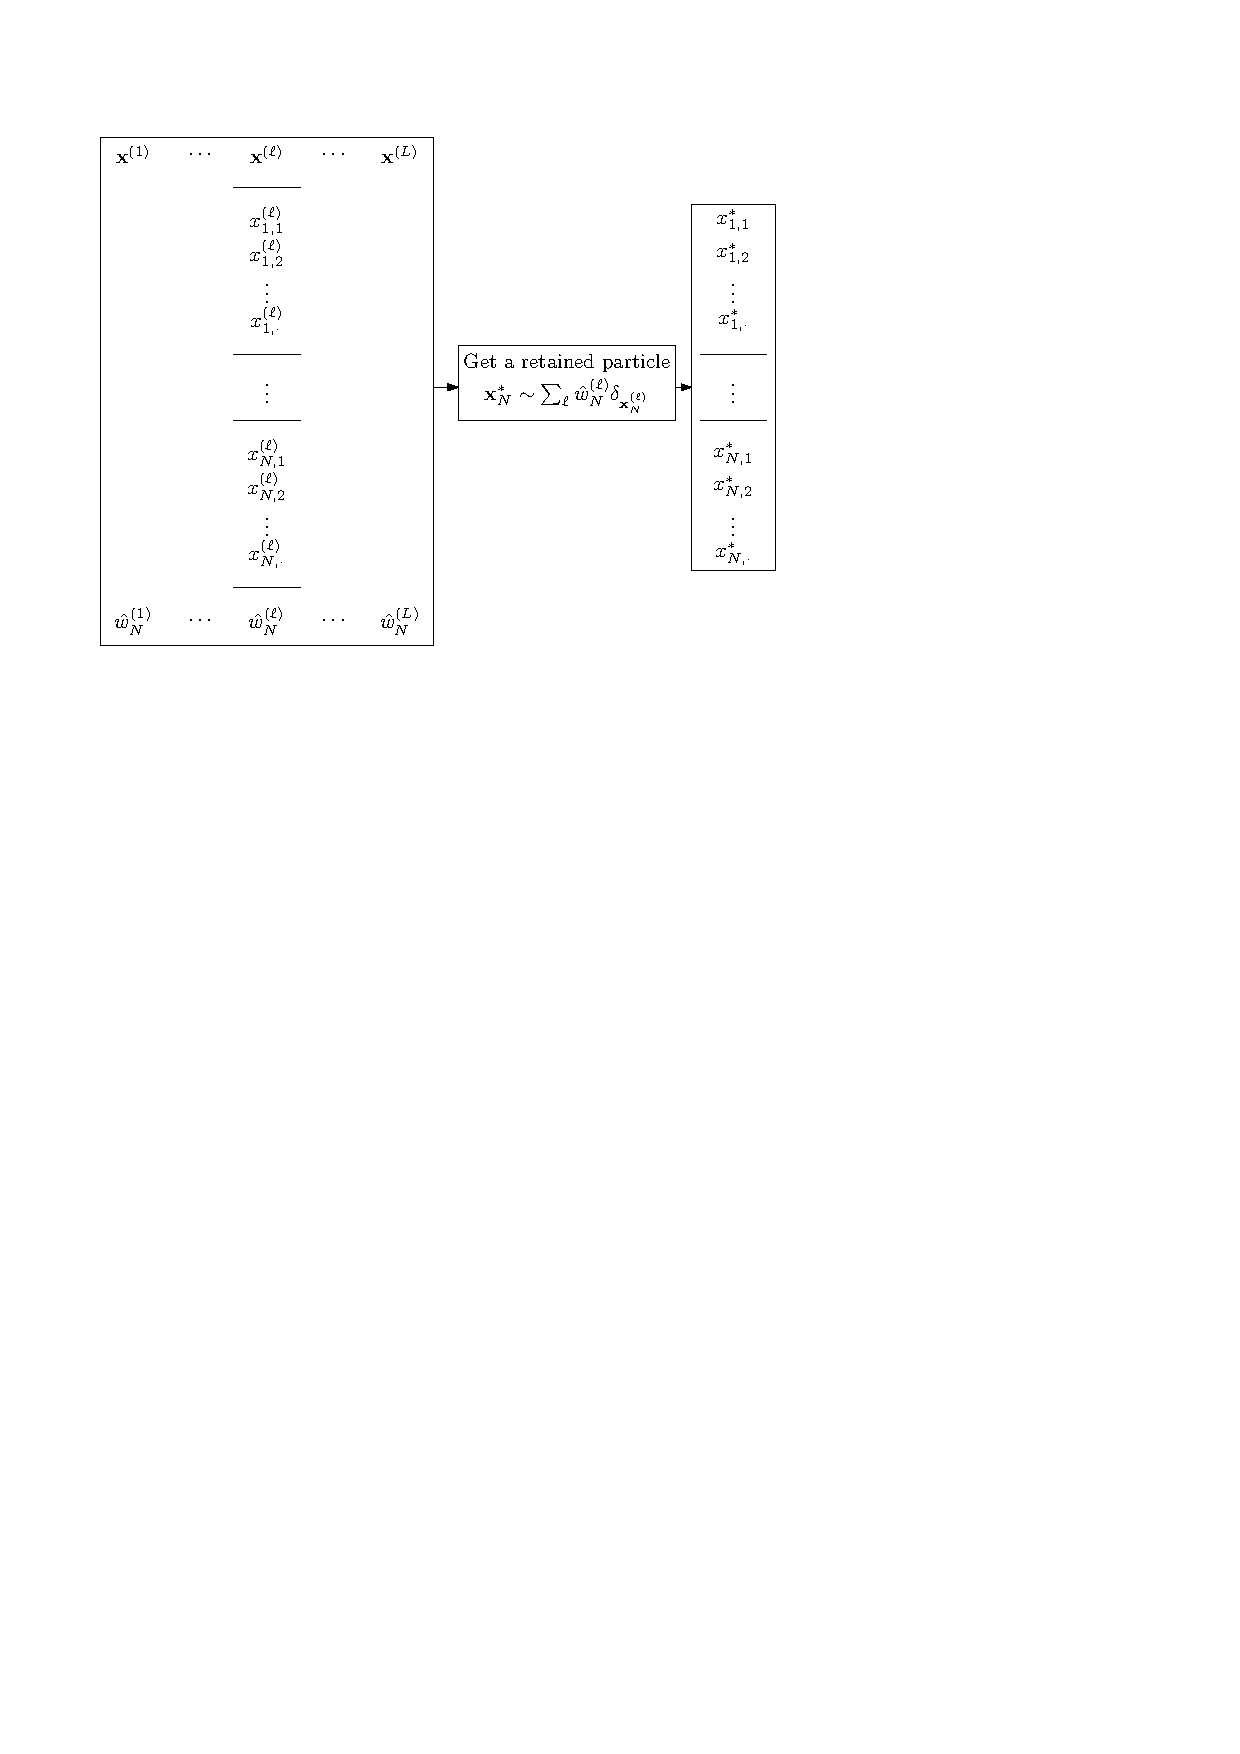
\includegraphics[scale=0.75]{pprog/how/figures/pgibbs/pgibbs1}
\caption{Initialisation of the Particle Gibbs sampler.}
\label{fig:pprog/how/figures/pgibbs1}
\end{figure}

\begin{figure}[!htb]
\centering
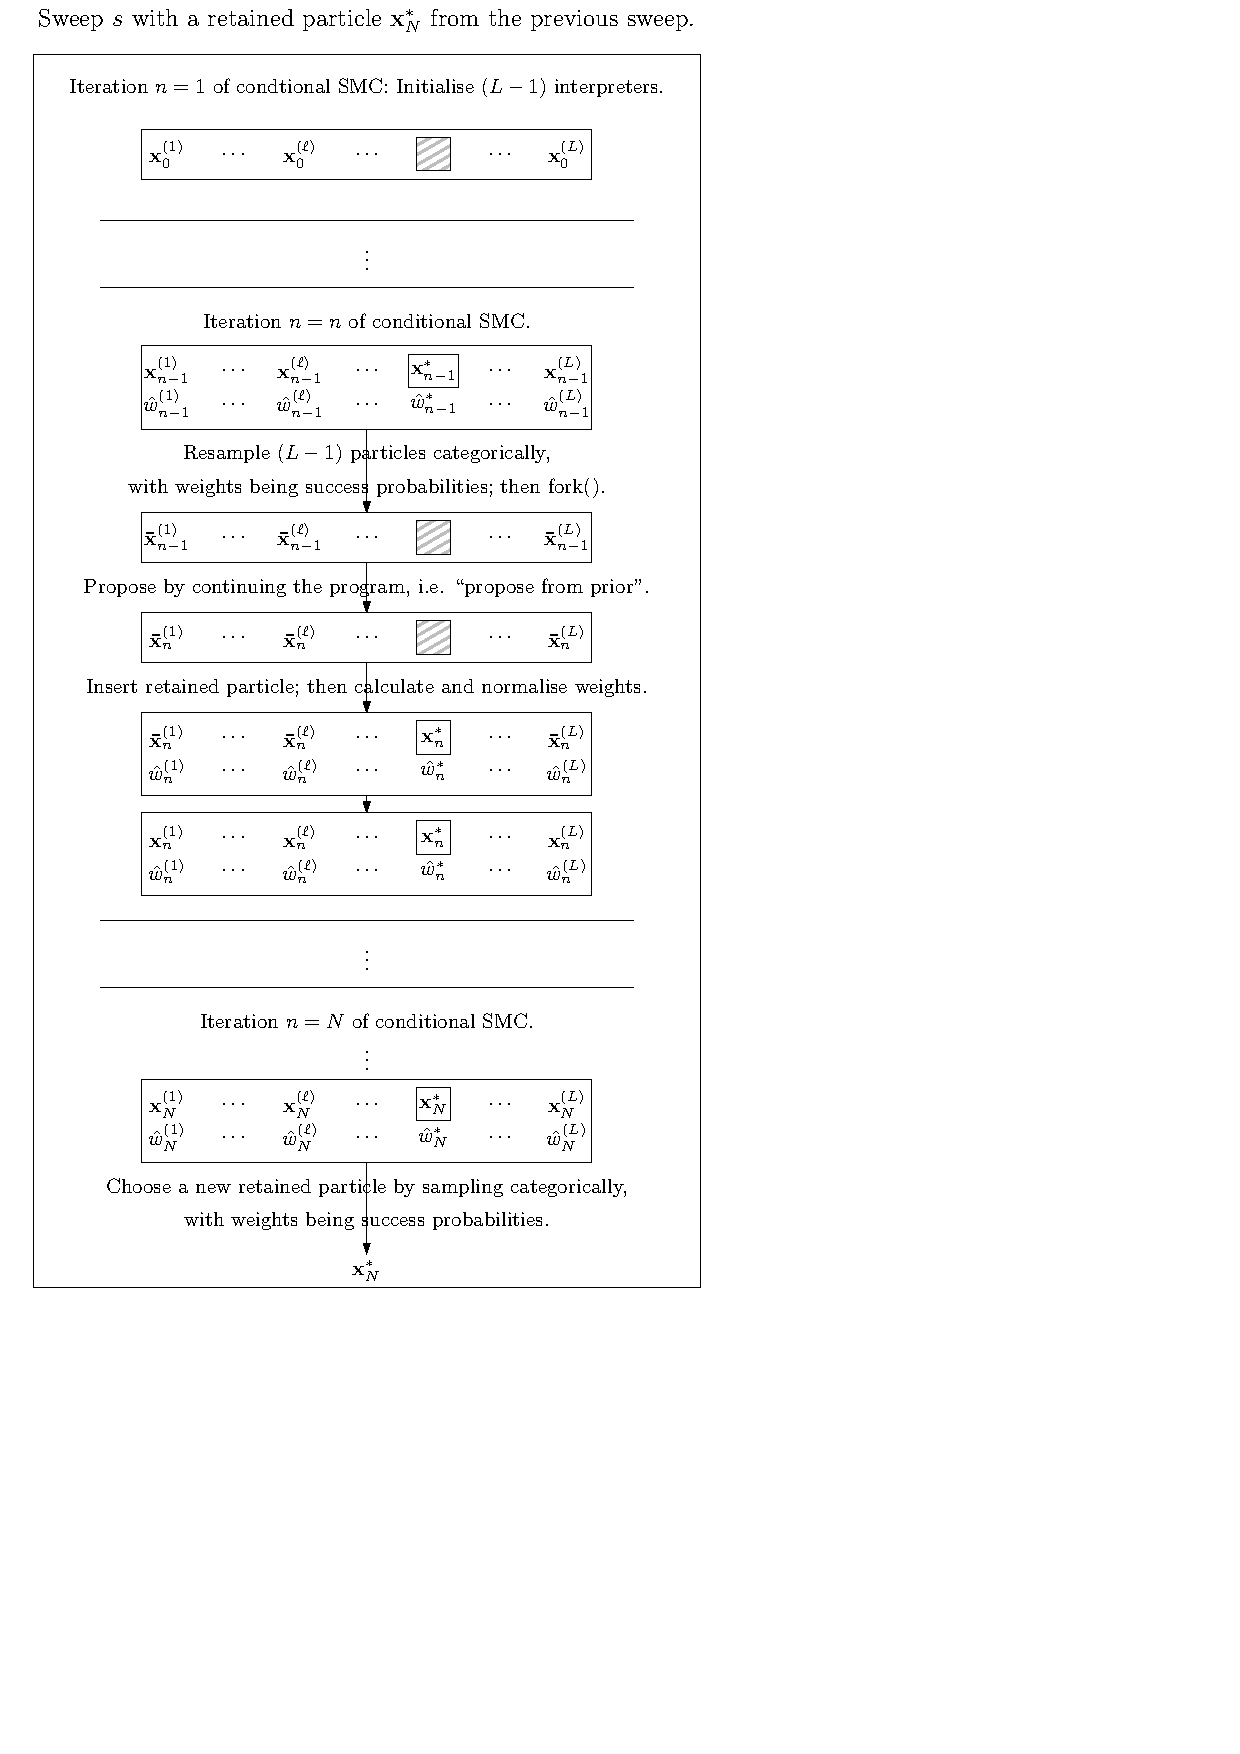
\includegraphics[scale=0.8]{pprog/how/figures/pgibbs/pgibbs2}
\caption{Sweep $s$ of the Particle Gibbs sampler.}
\label{fig:pprog/how/figures/pgibbs2}
\end{figure}